\documentclass{article}
\usepackage[utf8]{inputenc}
\usepackage[T1]{fontenc}
\usepackage[utf8]{inputenc}
\usepackage[norsk]{babel}
\usepackage{amsmath}
\usepackage{hyperref}
\usepackage{enumerate}
\usepackage{graphicx}
\usepackage{listings}
\usepackage{color}
\usepackage{gensymb}
\usepackage{verbatim}
\usepackage{float}
\usepackage{fancyvrb}
\usepackage{subfigure} 

\definecolor{codegreen}{rgb}{0,0.6,0}
\definecolor{codegray}{rgb}{0.5,0.5,0.5}
\definecolor{codepurple}{rgb}{0.58,0,0.82}
\definecolor{backcolour}{rgb}{0.95,0.95,0.92}
\setlength{\parindent}{0pt}
\lstdefinestyle{mystyle}{
    backgroundcolor=\color{backcolour},
    commentstyle=\color{codegreen},
    keywordstyle=\color{magenta},
    numberstyle=\tiny\color{codegray},
    stringstyle=\color{codepurple},
    basicstyle=\footnotesize,
    breakatwhitespace=false,
    breaklines=true,
    captionpos=b,
    keepspaces=true,
    numbers=left,
    numbersep=5pt,
    showspaces=false,
    showstringspaces=false,
    showtabs=false,
tabsize=2}
\lstset{style=mystyle}
\renewcommand{\thesubsection}{\thesection.\alph{subsection}}




\title{Ukeoppgaver}
\author{Mathias Kirkerød / mathiaki}
\date{\today}

\begin{document}

\maketitle
\newpage
\section{}
Matlab kode:
\begin{verbatim}
%% Oppgave 1 

r = [0 0.25, 0.5, 0.75, 1.0];
L = 128;

t1 = tukeywin(L,r(1));
t2 = tukeywin(L,r(2));
t3 = tukeywin(L,r(3));
t4 = tukeywin(L,r(4));
t5 = tukeywin(L,r(5));

wvtool(t1)
wvtool(t2)
wvtool(t3)
wvtool(t4)
wvtool(t5)



%% Oppgave 2

F_l=40;
F_h=60;
K=10;

t=linspace(-100,100,500);
k=1:K;
F_k=F_l+(k-1)*(F_h-F_l)/(K-1);
x_c=0;
for i=F_k
    x_c=x_c+cos(2*pi*i*t);
    
end
%plot(t,fft(x_c))

w_c=tukeywin(L,r(1));
xhat_c=0;
for i=F_k
    xhat_c=xhat_c+w_c*cos(2*pi*i*t);
    
end

plot(t,fft(xhat_c))


%% Oppgave 3


non_d=linspace(1,2,10000);
F_s=20;

A=1;
T=1;
for n=1:10
    h_c(n)=A*(exp(-A*non_d(n*1000)))^n;
end
h_C=A*(exp(-A*non_d)).^non_d;

figure(1)
stem(h_c)
ax1 = gca; % current axes
ax1.XColor = 'r';
ax1.YColor = 'r';
ax1_pos = get(ax1,'Position');
ax2 = axes('Position',ax1_pos,...
    'XAxisLocation','top',...
    'YAxisLocation','right',...
    'Color','none');
ax1_pos = ax1.Position; % position of first axes
plot(h_C,'Parent',ax2,'Color','k')



\end{verbatim}
\newpage
\subsubsection{assignment 1}
\begin{figure}[h!]
    \centering
    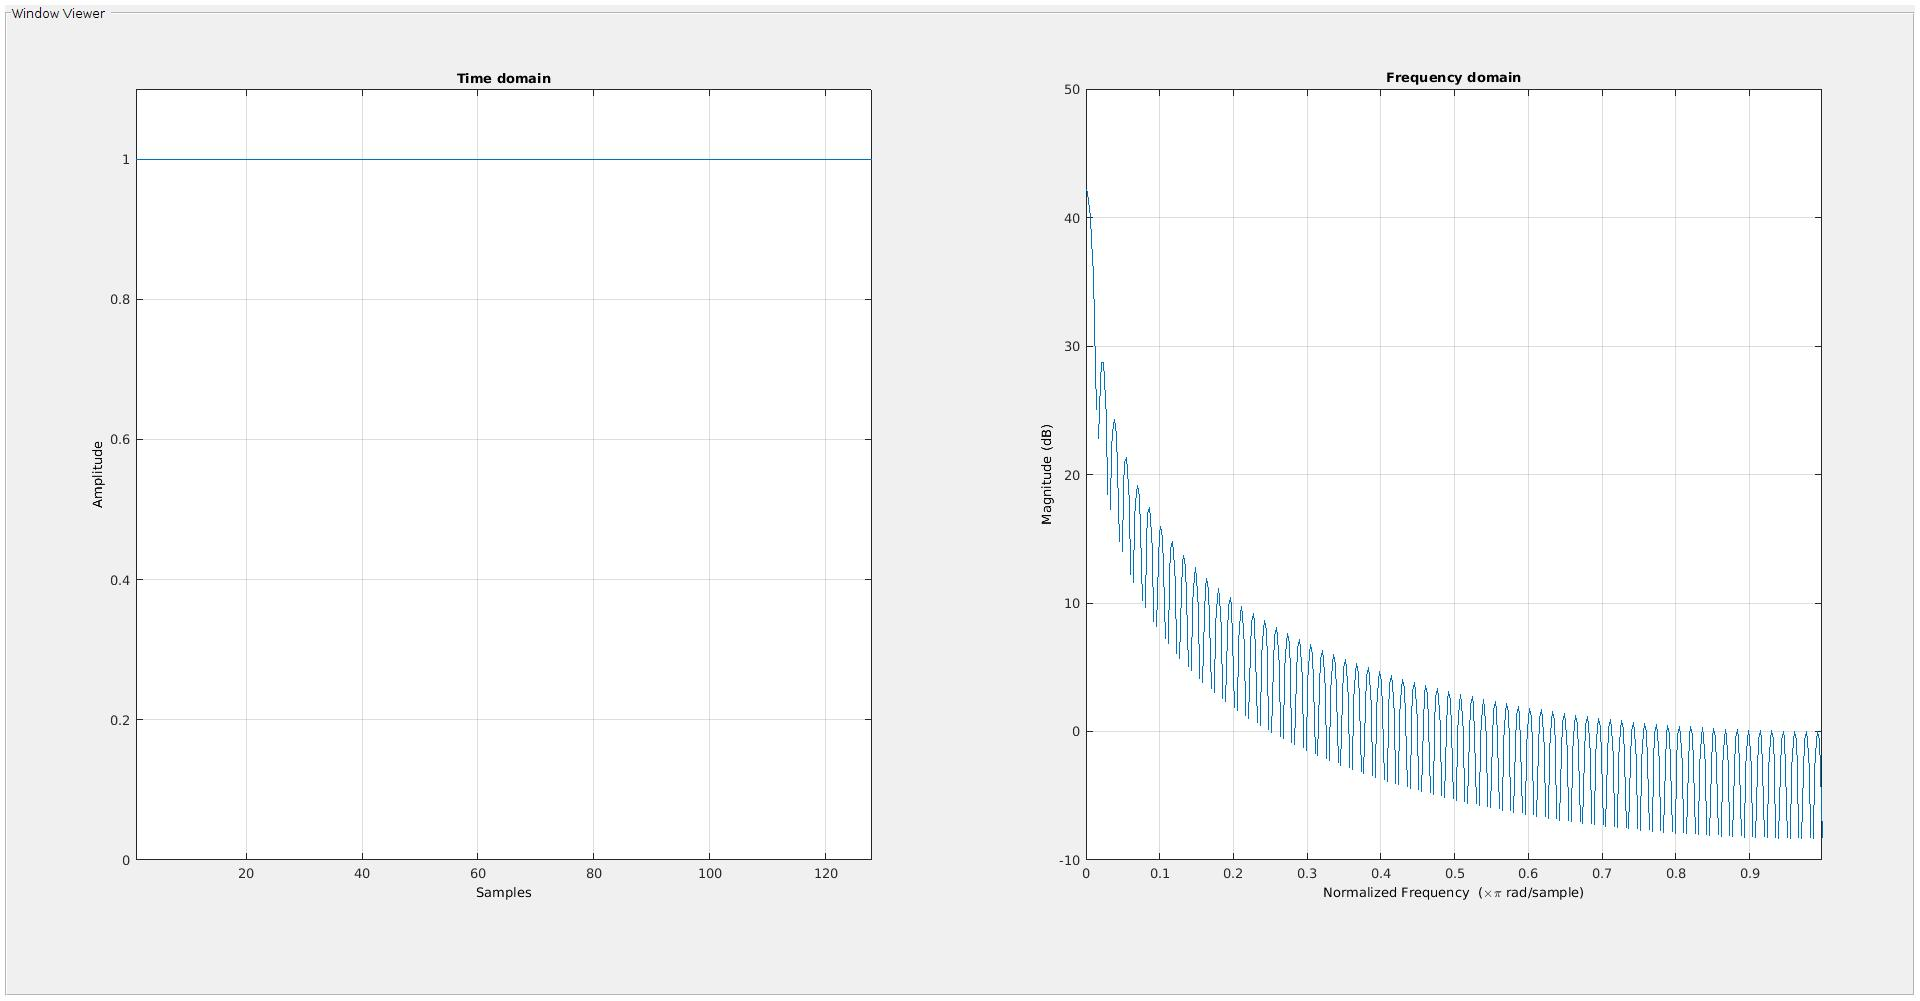
\includegraphics[scale=0.13]{fig1.jpg}
    \caption{plot1}
    \label{fig:plot1}
\end{figure}

\begin{figure}[h!]
    \centering
    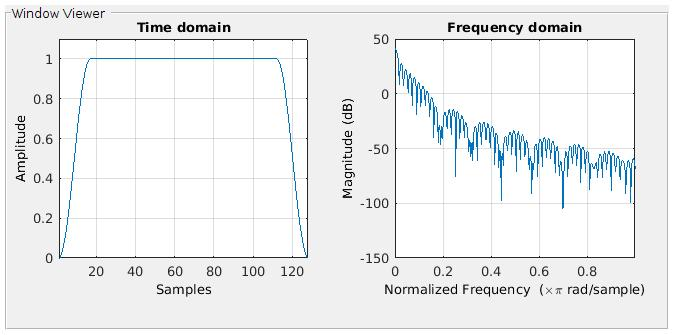
\includegraphics[scale=0.4]{fig2.jpg}
    \caption{plot2}
    \label{fig:plot2}
\end{figure}

\begin{figure}[h!]
    \centering
    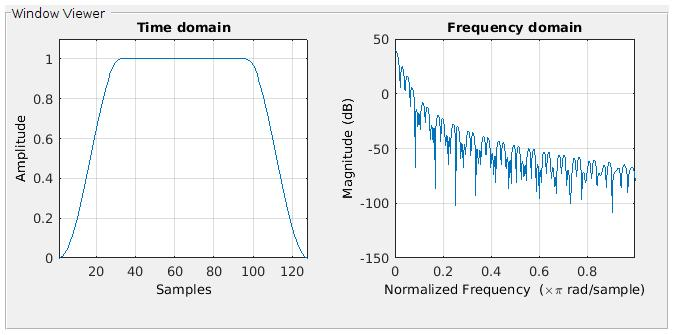
\includegraphics[scale=0.4]{fig3.jpg}
    \caption{plot3}
    \label{fig:plot3}
\end{figure}


\begin{figure}[h!]
    \centering
    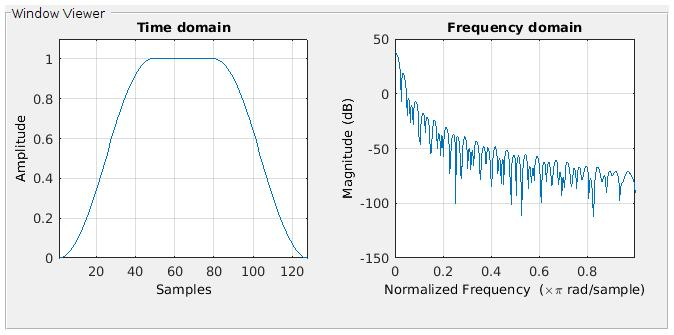
\includegraphics[scale=0.4]{fig4.jpg}
    \caption{plot3}
    \label{fig:plot3}
\end{figure}


\begin{figure}[h!]
    \centering
    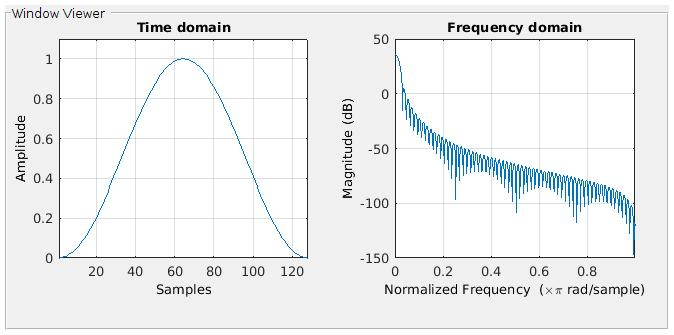
\includegraphics[scale=0.4]{fig5.jpg}
    \caption{plot3}
    \label{fig:plot3}
\end{figure}
\newpage
\newpage
\newpage

\subsubsection{assignment 2}


\begin{figure}[h!]
    \centering
    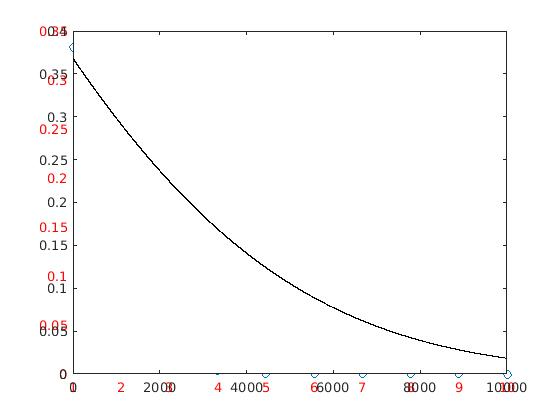
\includegraphics[scale=0.5]{fig6.jpg}
    \caption{plot3}
    \label{fig:plot3}
\end{figure}

\newpage
\subsubsection{assignment 3}
\begin{figure}[h!]
    \centering
    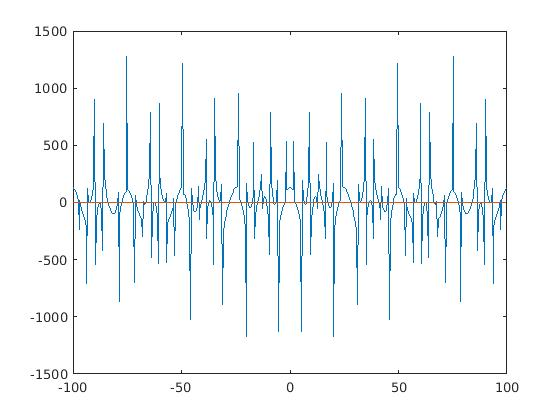
\includegraphics[scale=0.5]{fig7.jpg}
    \caption{plot3}
    \label{fig:plot3}
\end{figure}


\end{document}